\section{Funktionen und deren Eigenschaften}
\subsection{Elementare Eigenschaften von Funktionen}
\subsubsection{Nullstellen}
\begin{frame}{Nullstellen}
	\begin{definition}
		Die Funktion $y=f(x)$ besitzt an der Stelle $x_{0}$ eine \textbf{Nullstelle}, wenn
		\[
			f(x_{0}) = 0
		\]
		ist.
	\end{definition}
\begin{bemerkung}
			In der Nullstelle $x_{0}$ berührt oder schneidet der Funktionsgraph die x-Achse.
\end{bemerkung}

\end{frame}
\begin{frame}{Nullstelle einer linearen Funktion}
\begin{example}
	Die lineare Funktion $y = x - 2$ hat eine Nullstelle bei $x_{0}= 2$ und schneidet die x-Achse.
	\definecolor{qqwuqq}{rgb}{0.,0.39215686274509803,0.}
	\definecolor{qqwuqq}{rgb}{0.,0.39215686274509803,0.}
	\begin{tikzpicture}[line cap=round,line join=round,>=triangle 45,x=0.5cm,y=0.4cm]
	\draw[->,color=black] (-4.3,0.) -- (14.62,0.);
	\foreach \x in {-4.,-3.,-2.,-1.,1.,2.,3.,4.,5.,6.,7.,8.,9.,10.,11.,12.,13.,14.}
	\draw[shift={(\x,0)},color=black] (0pt,2pt) -- (0pt,-2pt) node[below] {\footnotesize $\x$};
	\draw[->,color=black] (0.,-7.36) -- (0.,6.3);
	\foreach \y in {-7.,-6.,-5.,-4.,-3.,-2.,-1.,1.,2.,3.,4.,5.,6.}
	\draw[shift={(0,\y)},color=black] (2pt,0pt) -- (-2pt,0pt) node[left] {\footnotesize $\y$};
	\draw[color=black] (0pt,-10pt) node[right] {\footnotesize $0$};
	\clip(-4.3,-7.36) rectangle (14.62,6.3);
	\draw[line width=1.2pt,color=qqwuqq,smooth,samples=100,domain=-4.300000000000001:14.620000000000005] plot(\x,{(\x)-2.0});
	\begin{scriptsize}
	\draw[color=qqwuqq] (-4.14,-6.28) node {$f$};
	\end{scriptsize}
	\end{tikzpicture}
	\end{example}
\end{frame}

\begin{frame}{Nullstelle einer quadratischen Funktion}
	\begin{example}
		Die quadratische Funktion 
		\[
			f(x)=(x-1)^2
		\]
		besitzt eine Nullstelle bei $x=1$ und berührt dort die x-Achse.
		\definecolor{ccqqqq}{rgb}{0.8,0.,0.}
		\begin{tikzpicture}[line cap=round,line join=round,>=triangle 45,x=0.5cm,y=0.25cm]
		\draw[->,color=black] (-4.3,0.) -- (14.62,0.);
		\foreach \x in {-4.,-3.,-2.,-1.,1.,2.,3.,4.,5.,6.,7.,8.,9.,10.,11.,12.,13.,14.}
		\draw[shift={(\x,0)},color=black] (0pt,2pt) -- (0pt,-2pt) node[below] {\footnotesize $\x$};
		\draw[->,color=black] (0.,-7.36) -- (0.,6.3);
		\foreach \y in {-7.,-6.,-5.,-4.,-3.,-2.,-1.,1.,2.,3.,4.,5.,6.}
		\draw[shift={(0,\y)},color=black] (2pt,0pt) -- (-2pt,0pt) node[left] {\footnotesize $\y$};
		\draw[color=black] (0pt,-10pt) node[right] {\footnotesize $0$};
		\clip(-4.3,-7.36) rectangle (14.62,6.3);
		\draw[line width=1.2pt,color=ccqqqq,smooth,samples=100,domain=-4.300000000000001:14.620000000000005] plot(\x,{((\x)-1.0)^(2.0)});
		\begin{scriptsize}
		\draw[color=ccqqqq] (-1.24,6.14) node {$f$};
		\end{scriptsize}
		\end{tikzpicture}
		Diese Nullstelle wird auch als \textbf{doppelte Nullstelle} bezeichnet, weil zwei Terme $x-1$ und $x-1$ gleichzeitig null werden.
	\end{example}
\end{frame}

\begin{frame}{Nullstellen periodischer Funktionen}
	\begin{example}
		Die Funktion $f(x)=\sin(x)$ hat unendlich viele Nullstellen. Die Nullstellen sind an den Stellen $x_{i} = i \pi$ für $i \in \mathbb{Z}$.
		\definecolor{qqqqff}{rgb}{0.,0.,1.}
		\begin{tikzpicture}[line cap=round,line join=round,>=triangle 45,x=0.5cm,y=0.9cm]
		\draw[->,color=black] (-4.28,0.) -- (14.6,0.);
		\foreach \x in {-4.,-3.,-2.,-1.,1.,2.,3.,4.,5.,6.,7.,8.,9.,10.,11.,12.,13.,14.}
		\draw[shift={(\x,0)},color=black] (0pt,2pt) -- (0pt,-2pt) node[below] {\footnotesize $\x$};
		\draw[->,color=black] (0.,-3.22) -- (0.,2.98);
		\foreach \y in {-3.,-2.5,-2.,-1.5,-1.,-0.5,0.5,1.,1.5,2.,2.5}
		\draw[shift={(0,\y)},color=black] (2pt,0pt) -- (-2pt,0pt) node[left] {\footnotesize $\y$};
		\draw[color=black] (0pt,-10pt) node[right] {\footnotesize $0$};
		\clip(-4.28,-3.22) rectangle (14.6,2.98);
		\draw[line width=1.2pt,color=qqqqff,smooth,samples=100,domain=-4.280000000000001:14.600000000000003] plot(\x,{sin(((\x))*180/pi)});
		\begin{scriptsize}
		\draw[color=qqqqff] (-4.120338266384779,0.7741434846266446) node {$h$};
		\end{scriptsize}
		\end{tikzpicture}
	\end{example}
\end{frame}

\subsubsection{Symmetrie}
\begin{frame}{Symmetrie}
	\begin{definition}
		Eine Funktion f heißt \textbf{gerade} bzw. \textbf{achsensymmetrisch}, wenn  die Bedingung
		\[
			f(x) = f(-x) \qquad \forall x \in D
		\]
		erfüllt ist.
	\end{definition}
	\begin{bemerkung}
		Streng genommen nennt man nur die Funktion \textbf{gerade}, der dazugehörige Funktionsgraph ist dann \textbf{achsensymmetrisch} (zur y-Achse).
		
		$D$ bezeichnet den Definitionsbereich der Funktion, das heißt: $D$ ist die Menge der Zahlen $x$, für die $f(x)$ überhaupt definiert ist.
		
		$\forall$ ist das Symbol für "{}für alle"{}.
	\end{bemerkung}
\end{frame}

\begin{frame}{Symmetrie einer quadratischen Funktion}
	\begin{example}
		Die Funktion $f(x)=x^2$ ist gerade\footnote{Das liegt auch daran, dass nur (ein) gerade(r) Exponent(en) vorkommen!}. 
		\definecolor{ffvvqq}{rgb}{1.,0.3333333333333333,0.}
		\begin{tikzpicture}[line cap=round,line join=round,>=triangle 45,x=2cm,y=1.5cm]
		\draw[->,color=black] (-2.1844397463002125,0.) -- (2.246173361522198,0.);
		\foreach \x in {-2.,-1.8,-1.6,-1.4,-1.2,-1.,-0.8,-0.6,-0.4,-0.2,0.2,0.4,0.6,0.8,1.,1.2,1.4,1.6,1.8,2.,2.2}
		\draw[shift={(\x,0)},color=black] (0pt,2pt) -- (0pt,-2pt) node[below] {\footnotesize $\x$};
		\draw[->,color=black] (0.,-0.21531478770132104) -- (0.,2.9618448023426045);
		\foreach \y in {-0.2,0.2,0.4,0.6,0.8,1.,1.2,1.4,1.6,1.8,2.,2.2,2.4,2.6,2.8}
		\draw[shift={(0,\y)},color=black] (2pt,0pt) -- (-2pt,0pt) node[left] {\footnotesize $\y$};
		\draw[color=black] (0pt,-10pt) node[right] {\footnotesize $0$};
		\clip(-2.1844397463002125,-0.21531478770132104) rectangle (2.246173361522198,2.9618448023426045);
		\draw[line width=1.2pt,color=ffvvqq,smooth,samples=100,domain=-2.1844397463002125:2.246173361522198] plot(\x,{(\x)^(2.0)});
		\begin{scriptsize}
		\draw[color=ffvvqq] (-1.6598851288836058,2.9292824053729007) node {$f$};
		\end{scriptsize}
		\end{tikzpicture}
	\end{example}
\end{frame}

\begin{frame}{Symmetrie der Kosinus-Funktion}
	\begin{example}
		Die Funktion $f(x)=\cos x$ ist gerade.
		\definecolor{zzttff}{rgb}{0.6,0.2,1.}
		\begin{tikzpicture}[line cap=round,line join=round,>=triangle 45,x=0.45cm,y=1.0cm]
		\draw[->,color=black] (-10.897842255586003,0.) -- (11.532136602764956,0.);
		\foreach \x in {-10.,-8.,-6.,-4.,-2.,2.,4.,6.,8.,10.}
		\draw[shift={(\x,0)},color=black] (0pt,2pt) -- (0pt,-2pt) node[below] {\footnotesize $\x$};
		\draw[->,color=black] (0.,-2.4276582084565703) -- (0.,1.9494486572603942);
		\foreach \y in {-2.,-1.5,-1.,-0.5,0.5,1.,1.5}
		\draw[shift={(0,\y)},color=black] (2pt,0pt) -- (-2pt,0pt) node[left] {\footnotesize $\y$};
		\draw[color=black] (0pt,-10pt) node[right] {\footnotesize $0$};
		\clip(-10.897842255586003,-2.4276582084565703) rectangle (11.532136602764956,1.9494486572603942);
		\draw[line width=1.2pt,color=zzttff,smooth,samples=100,domain=-10.897842255586003:11.532136602764956] plot(\x,{cos(((\x))*180/pi)});
		\begin{scriptsize}
		\draw[color=zzttff] (-10.708159559109461,-0.18463126409209377) node {$cos$};
		\end{scriptsize}
		\end{tikzpicture}
		
	\end{example}
\end{frame}

\begin{frame}{Symmetrie}
	\begin{definition}
		Eine Funktion f heißt \textbf{ungerade} bzw. \textbf{punktsymmetrisch}, wenn  die Bedingung
		\[
		f(x) = - f(-x) \qquad \forall x \in D
		\]
		erfüllt ist.
	\end{definition}
	\begin{bemerkung}
		Streng genommen nennt man wieder nur die Funktion \textbf{ungerade}, der dazugehörige Funktionsgraph ist dann \textbf{punktsymmetrisch} (zum Ursprung).
	\end{bemerkung}
\end{frame}

\begin{frame}{Symmetrie einer kubischen Funktion}
	\begin{example}
		Die Funktion $f(x)=x^3$ ist ungerade\footnote{Das liegt auch daran, dass nur (ein) ungerade(r) Exponent(en) vorkommen!}.
		\begin{tikzpicture}[line cap=round,line join=round,>=triangle 45,x=3.5cm,y=8.0cm]
		\draw[->,color=black] (-1.4479556964005578,0.) -- (1.5057863754810505,0.);
		\foreach \x in {-1.4,-1.2,-1.,-0.8,-0.6,-0.4,-0.2,0.2,0.4,0.6,0.8,1.,1.2,1.4}
		\draw[shift={(\x,0)},color=black] (0pt,2pt) -- (0pt,-2pt) node[below] {\footnotesize $\x$};
		\draw[->,color=black] (0.,-0.3408915185936749) -- (0.,0.23551761598633617);
		\foreach \y in {-0.3,-0.25,-0.2,-0.15,-0.1,0.15,0.2}
		\draw[shift={(0,\y)},color=black] (2pt,0pt) -- (-2pt,0pt) node[left] {\footnotesize $\y$};
		\draw[color=black] (0pt,-10pt) node[right] {\footnotesize $0$};
		\clip(-1.4479556964005578,-0.3408915185936749) rectangle (1.5057863754810505,0.23551761598633617);
		\draw[line width=1.2pt,smooth,samples=100,domain=-1.4479556964005578:1.5057863754810505] plot(\x,{(\x)^(3.0)});
		\begin{scriptsize}
		\draw[color=black] (-0.6580014213624532,-0.3299203344801462) node {$x^3$};
		\end{scriptsize}
		\end{tikzpicture}
		 
	\end{example}
\end{frame}

\begin{frame}{Symmetrie der Sinus-Funktion}
	\begin{example}
		Die Funktion $f(x)=\sin x$ ist ungerade.
		\definecolor{zzttff}{rgb}{0.6,0.2,1.}
		\begin{tikzpicture}[line cap=round,line join=round,>=triangle 45,x=0.45cm,y=1.0cm]
		\draw[->,color=black] (-10.897842255586003,0.) -- (11.532136602764956,0.);
		\foreach \x in {-10.,-8.,-6.,-4.,-2.,2.,4.,6.,8.,10.}
		\draw[shift={(\x,0)},color=black] (0pt,2pt) -- (0pt,-2pt) node[below] {\footnotesize $\x$};
		\draw[->,color=black] (0.,-2.4276582084565703) -- (0.,1.9494486572603942);
		\foreach \y in {-2.,-1.5,-1.,-0.5,0.5,1.,1.5}
		\draw[shift={(0,\y)},color=black] (2pt,0pt) -- (-2pt,0pt) node[left] {\footnotesize $\y$};
		\draw[color=black] (0pt,-10pt) node[right] {\footnotesize $0$};
		\clip(-10.897842255586003,-2.4276582084565703) rectangle (11.532136602764956,1.9494486572603942);
		\draw[line width=1.2pt,color=zzttff,smooth,samples=100,domain=-10.897842255586003:11.532136602764956] plot(\x,{sin(((\x))*180/pi)});
		\begin{scriptsize}
		\draw[color=zzttff] (-10.708159559109461,-0.18463126409209377) node {$sin$};
		\end{scriptsize}
		\end{tikzpicture}
		
	\end{example}
\end{frame}


\subsubsection{Monotonie}
\begin{frame}{Monotonie}
	\begin{definition}
		Eine Funktion $y=f(x)$ heißt
		\begin{itemize}
			\item \textbf{monoton wachsend}, wenn $\forall  x_{1}, x_{2} \in D(f) \mbox{ mit } x_{1} < x_{2}  \qquad f(x_{1}) \leq f(x_{2})$ gilt
			\item \textbf{streng monoton wachsend}, wenn $\forall  x_{1}, x_{2} \in D(f) \mbox{ mit } x_{1} < x_{2}  \qquad f(x_{1}) < f(x_{2})$ gilt
			\item \textbf{monoton fallend}, wenn $\forall  x_{1}, x_{2} \in D(f) \mbox{ mit } x_{1} < x_{2}  \qquad f(x_{1}) \geq f(x_{2})$ gilt
			\item \textbf{streng monoton fallend}, wenn $\forall  x_{1}, x_{2} \in D(f) \mbox{ mit } x_{1} < x_{2}  \qquad f(x_{1}) > f(x_{2})$ gilt
						
		\end{itemize}
	\end{definition}
\end{frame}

\begin{frame}{Beispiele - Monotonie}
	\begin{example}
		\begin{itemize}
			\item Jede lineare Funktion $y = a x + b$ mit $a>0$ ist streng monoton wachsend.
			\item Jede lineare Funktion $y = a x + b$ mit $a<0$ ist streng monoton fallend.
			\item Die kubische Funktion $y=x^3$ ist streng monoton wachsend.
			\item Die Exponentialfunktion $y=e^{x}$ ist streng monoton wachsend.
			\item Die Exponentialfunktion $y=e^{-x}$ ist streng monoton fallend.
		\end{itemize}
	\end{example}
\end{frame}

\begin{frame}{Bemerkung zur Monotonie}
	\begin{bemerkung}
		Falls die Funktion $y=f(x)$
		\begin{itemize}
			\item streng monoton wachsend ist, gilt $\frac{f(x_{2}) - f(x_{1})}{x_{2} - x_{1}} > 0$ 
			\item streng monoton fallend ist, gilt
			$\frac{f(x_{2}) - f(x_{1})}{x_{2} - x_{1}} < 0$
			\item monoton wachsend ist, gilt
			$\frac{f(x_{2}) - f(x_{1})}{x_{2} - x_{1}} \geq 0$ 
			\item monoton fallend ist, gilt
			$\frac{f(x_{2}) - f(x_{1})}{x_{2} - x_{1}} \leq 0$ 
		\end{itemize}
		$\forall x_{1} \neq x_{2} \in D(f)$.
	\end{bemerkung}
\end{frame}

\subsubsection{Periodizität}
\begin{frame}{Periodizität}
	\begin{definition}
		Eine Funktion $y=f(x)$ heißt periodisch mit der Periode $T$, wenn für alle $x \in D(f)$ und für alle $n \in \mathbb{Z}$ sowohl
		\begin{itemize}
			\item $x+n \cdot T \in D(f)$ ist als auch
			\item $f(x+n \cdot T) = f(x)$ gilt.   
		\end{itemize} 
	\end{definition}
	\begin{example}
		Die Funktion $y = \sin(x)$ ist periodisch mit der Periode $T=2 \pi$, denn
		\[
			\sin(x) = \sin( x + n \cdot 2 \pi) \qquad \forall n\in \mathbb{Z}, x \in  \mathbb{R}
		\]
	\end{example}
\end{frame}

\subsection{Grenzwerte von Funktionen}
\subsubsection{Grenzwerte für $x \to x_{0}$}
\begin{frame}{Grenzwerte für $x \to x_{0}$}
	\begin{definition}
		Eine Funktion $y = f(x)$ sei in einer Umgebung von $x_{0} \in \mathbb{R}$ definiert\footnote{D.h. anschaulich, dass jeder Punkt $x$, der nach genug an $x_{0}$ liegt, im Definitionsbereich der Funktion liegt.}. Wenn für jede beliebige Folge $(x_{n})$ mit $\lim_{n \to \infty}x_{n} = x_{0}$ gilt:
	\[
		\lim_{n \to \infty} f(x_{n}) = g
	\]
	so heißt $g$ der Grenzwert der Funktion $f$ an der Stelle $x_{0}$ und man schreibt:
	\[
		\lim_{x \to x_{0}} f(x) = g
	\]
	\end{definition}
\end{frame}	

\begin{frame}{Grenzwerte einer Funktion für $x \to x_{0}$}
	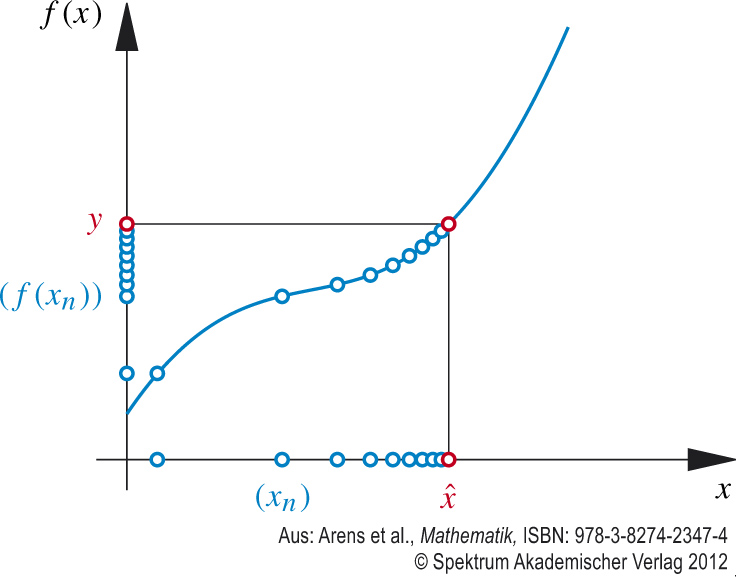
\includegraphics[width=10cm]{stetigkeit.jpg}
\end{frame}
\begin{frame}{Grenzwerte einer Funktion für $x \to x_{0}$}
	\begin{bemerkung}
		\begin{itemize}
			\item Der Punkt $x_{0}$ muss dabei nicht unbedingt im Definitionsbereich der Funktion liegen.
			\item Man unterscheidet manchmal (siehe nächste Folie) noch, ob der Grenzwert nur für $x < x_{0}$ bzw. $x > x_{0}$ betrachtet wird. Die Definition hier verlangt noch, dass es für \textbf{jede} Folge gilt.
		\end{itemize}
	\end{bemerkung}
\end{frame}

\begin{frame}{Grenzwerte einer Funktion für $x \to x_{0}$}
	\begin{definition}
		Beschränkt man die Folge $x_{n}$ in der Definition des Grenzwertes (s.o.) auf Folgen mit $x_{n}<x_{0}$ und existiert dieser Grenzwert, so nennt man diesen den \textbf{linksseitigen Grenzwert} von $f$ an der Stelle $x_{0}$ und schreibt:
		\[
			\lim_{x \nearrow x_{0}} f(x) = \lim_{x \to x_{0} - 0} f(x) = g_{l}
		\]
	\end{definition}
		\begin{definition}
			Beschränkt man die Folge $x_{n}$ in der Definition des Grenzwertes (s.o.) auf Folgen mit $x_{n}>x_{0}$ und existiert dieser Grenzwert, so nennt man diesen den \textbf{rechtsseitigen Grenzwert} von $f$ an der Stelle $x_{0}$ und schreibt:
			\[
			\lim_{x \searrow x_{0}} f(x) =\lim_{x \to x_{0} + 0} f(x) = g_{r}
			\]
		\end{definition}
\end{frame}
\begin{frame}{Zusammenhang der Grenzwertbegriffe}
	\begin{bemerkung}
		Offenbar existiert der Grenzwert einer Funktion $f$ an der Stelle $x_{0}$ genau dann, wenn sowohl der rechtsseitige als auch der linksseitige Grenzwert existieren und die beiden übereinstimmen. Dann ist
		\[
			\lim_{x \to x_{0}} f(x) = \lim_{x \nearrow x_{0}} f(x) = \lim_{x \searrow x_{0}} f(x)
		\]
	\end{bemerkung}
\end{frame}

\begin{frame}{Grenzwerte einer Funktion für $x \to x_{0}$}
	Für die Funktion
	\[
	f(x)=\begin{cases}
	0 & \text{ falls } x \leq 0 \\
	\sin(\frac{1}{x}) & \text{ falls } x>0
	\end{cases}
	\]
	existiert der rechtsseitige Grenzwert nicht!
	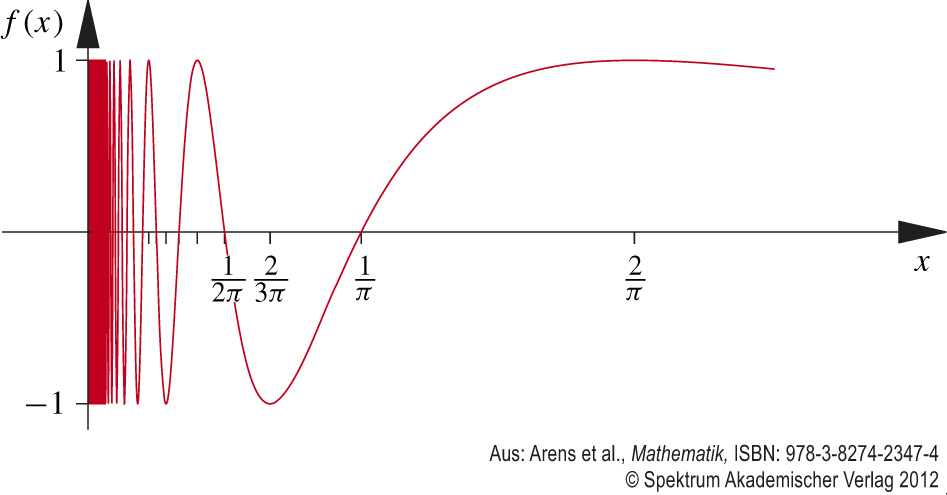
\includegraphics[width=9cm]{unstetig.jpg}
\end{frame}

\subsubsection{Grenzwerte für $x \to \pm \infty$}
\begin{frame}{Grenzwerte für $x \to \pm \infty$}
	\begin{definition}
		Für eine Funktion $y=f(x)$ definiert man
		\[
		\lim_{x \to \infty} f(x) = g \in \mathbb{R}
		\]
		wenn für alle Folgen $(x_{n})$ mit $x_{n} \to \infty$ der Grenzwert der Folge $f(x_{n})$ existiert und unabhängig von der Wahl der Folge gleich $g$ ist.
	\end{definition}
		\begin{definition}
			Für eine Funktion $y=f(x)$ definiert man
			\[
			\lim_{x \to -\infty} f(x) = g \in \mathbb{R}
			\]
			wenn für alle Folgen $(x_{n})$ mit $x_{n} \to -\infty$ der Grenzwert der Folge $f(x_{n})$ existiert und unabhängig von der Wahl der Folge gleich $g$ ist.
		\end{definition}	
\end{frame}

\subsection{Stetigkeit von Funktionen}
\begin{frame}{Stetigkeit}
	\begin{definition}
		Eine Funktion $f$ heißt \textbf{stetig an der Stelle $x_{0}$}, wenn sowohl der rechtsseitige als auch der linksseitige Grenzwert der Funktion an der Stelle $x_{0}$ existiert, beide gleich sind und der gemeinsame Grenzwert gleich $f(x_{0})$ ist, also:
		\[
			\lim_{x \to x_{0}} f(x) = \lim_{x \searrow x_{0}} f(x) = \lim_{x \nearrow x_{0}} f(x) = f(x_{0})
		\]
		ist.
		Stellen, an denen eine Funktion nicht stetig ist, nennt man \textbf{Unstetigkeitsstellen}.
	\end{definition}
\end{frame}	
\begin{frame}{Stetigkeit von Funktionen}
	\begin{theorem}
		Seien $f$ und $g$ in $x_{0}$ stetig und $c \in \mathbb{R}$ eine Konstante. Dann gilt:
		\begin{itemize}
			\item $f + g$, $f \cdot g$ und $c \cdot f$ sind stetig in $x_{0}$.
			\item Falls $g(x_{0}) \neq 0$, so ist auch $\frac{f}{g}$ stetig in $x_{0}$.
			\item $f^{r}$, d.h. die Funktion $x \mapsto \left( f(x) \right)^{r}$ für $r \in \mathbb{R}$ ist stetig in $x_{0}$, falls dort definiert.
			\item Falls $f$ im Punkt $g(x_{0})$ stetig ist, so ist auch $f \circ g$ stetig in $x_{0}$, d.h. die Hintereinanderausführung stetiger Funktionen ist stetig.
		\end{itemize}
	\end{theorem}
\end{frame}

\begin{frame}{Unstetigkeitsstellen - Sprungstellen}
		\begin{example}
			Falls sowohl der linksseitige als auch der rechtsseitige Grenzwert an der Stelle $x_{0}$ existieren, \textbf{aber verschieden sind}, nennt man die Unstetigkeitsstelle eine \textbf{Sprungstelle}.
			\[
			f(x) := \begin{cases}
			0 & \text{falls } x<0 \\
			1 & \text{falls } x\geq 0
			\end{cases}
			\] 
			hat an der Stelle $x_{0}=0$ eine Sprungstelle, weil
			\[
			\lim_{x \searrow 0} f(x) = 1 = f(0) \qquad\text{ aber }\qquad \lim_{x \nearrow 0} f(x) = 0 
			\] 
			Diese Funktion ist übrigens \textbf{rechtsseitig stetig}.
		\end{example}
\end{frame}

\begin{frame}{Unstetigkeitsstellen - hebbare Definitionslücken}
	\begin{example}
		Falls sowohl der linksseitige als auch der rechtsseitige Grenzwert an der Stelle $x_{0}$ existieren und gleich sind, die Funktion an der Stelle $x_{0}$ aber nicht definiert ist, nennt man die Unstetigkeitsstelle eine \textbf{hebbare Definitionslücke}.
		\[
		f(x) := \frac{x^2 - 1}{x-1}
		\] 
		hat an der Stelle $x_{0}=1$ eine hebbare Definitionslücke, weil
		\[
			\lim_{x \searrow 1} f(x) = \lim_{x \nearrow 1} f(x) = \lim_{x \to 1} f(x) = \lim_{x \to 1} \frac{x^2 - 1}{x-1} = \lim_{x \to 1} x+1 = 2
		\] 
		Man kann die Definitionslücke also beheben, indem man $f(1)=2$ setzt\footnote{Die Funktion wird dann \textbf{stetig ergänzt}.} und damit eine überall stetige Funktion erzeugt (die genauso aussieht wie die Funktion $f(x)=x+1)$).
	\end{example}
\end{frame}

\begin{frame}{Unstetigkeitsstellen - Polstellen}
	\begin{example}
		Falls mindestens einer der beiden (linksseitig und rechtsseitig) Grenzwerte einer Funktion $f$ an der Stelle $x_{0}$ uneigentlich (also $\infty$ oder $-\infty$) ist, nennt man die Unstetigkeitsstelle $x_{0}$ eine \textbf{Polstelle}.
		Es gibt \textbf{Polstellen ohne Vorzeichenwechsel}:
		\[
			\lim_{x \searrow x_{0}} f(x) = \lim_{x \nearrow x_{0}} f(x) = \pm \infty
		\] und \textbf{Polstellen mit Vorzeichenwechsel}:
		\[
		\lim_{x \searrow x_{0}} f(x) = \pm \infty \qquad \lim_{x \nearrow x_{0}} f(x) = \mp \infty
		\]
		Die Funktion
		\[
		f(x)=\frac{1}{x} 
		\]
		hat an der Stelle $x_{0}=0$ eine Polstelle mit Vorzeichenwechsel.
	\end{example}
\end{frame}

\begin{frame}{Beispiele stetiger Funktionen}
	\begin{example}
		\begin{itemize}
			\item Polynome sind auf ganz $\mathbb{R}$ stetig.
			\item Rationale Funktionen sind auf ihrem Definitionsbereich (also auf ganz $\mathbb{R}$, ausgenommen etwaige Nullstellen des Nennerpolynoms) stetig.
			\item Die Exponentialfunktion $f(x)=e^x$ ist stetig auf ganz $\mathbb{R}$.
			\item $\sin$ und $\cos$ sind stetig auf ganz $\mathbb{R}$.
			\item $\tan$ und $\cot$ sind stetig auf ihrem jeweiligen Definitionsbereich.
		\end{itemize}
	\end{example}
\end{frame}

\begin{frame}{Einschub - Horner-Schema}
	\begin{bemerkung}
		Das \textbf{Horner-Schema} ein Verfahren, mit dem man \textbf{für Polynome} sehr schnell \textbf{Funktionswerte berechnen} kann (und damit auch \textbf{überprüfen kann, ob eine vermutete Nullstelle tatsächlich eine ist}), und mit dem man für \textbf{einfache gebrochen-rationale Funktionen die Asymptote berechnen} kann.
	\end{bemerkung}
\end{frame}		
\begin{frame}{Horner-Schema zur Berechnung des Funktionswertes}
	\begin{example}
		Für die Funktion \[ f(x)=3x^{3} + 2x^{2} -5 x +10 \] berechnet man beispielsweise den Wert an der Stelle $x=2$ so:
		\[
		\horner{3,2,-5,10}{2}
		\]
	\end{example}
\end{frame}

\begin{frame}{Horner-Schema zur Überprüfung vermuteter Nullstellen}
		\begin{example}
			Für die Funktion $f(x)=x^{3} -9x^{2} +27x -27$ berechnet man beispielsweise den Wert an der Stelle $x=3$ so:
			\[
			\horner{1,-9,27,-27}{3}
			\]
			Das Ergebnis der Polynomdivision
			\[
			\left( x^{3} -9x^{2} +27x -27 \right) : (x-3) = x^2-6x+9
			\]
			kann man aus den entstandenen Koeffizienten des Horner-Schemas ablesen.
		\end{example}
\end{frame}

\begin{frame}{Horner-Schema zur Berechnung von Asymptoten}
	\begin{example}
		Für gebrochen-rationale Funktionen mit einem einzelnen Linearfaktor im Nenner kann man mit dem Horner-Schema sehr schnell die \textbf{Asymptote} ausrechnen:
		
		Für die Funktion
		\[
		f(x)=\frac{x^{2}-2x-10}{x-5}
		\]
		ist mit dem Horner-Schema für $x=5$ (die Nullstelle des Linearfaktors im Nenner)
		\[
		\horner{1,-2,-10}{5}
		\]
		und damit
		\[
		f(x)=\frac{x^{2}-2x-10}{x-5} = x+3 + \frac{5}{x-5}
		\]
	\end{example}
\end{frame}